\pagebreak
\subsection{Ground Support Equipment}\label{sec:4.9}
A laptop on the ground was connected to the experiment via the E-Link. A spare laptop was kept close-by should any problems arise with the main one. The ground support software included a simple GUI which enabled an operator to issue commands to the experiment such as reset, target selection, and moving to landing position. Compressed pictures could be received by the ground support software, which could be examined to verify nominal operation. The ground support software was written in C and Python, using GTK+ to build the GUI.

\begin{figure}[h]
	\centering
	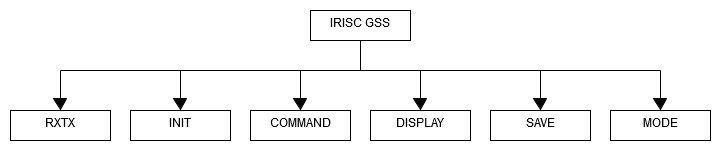
\includegraphics[width=\textwidth]{4-experiment-design/img/software/GSS-tree.png}
	\caption{Design tree of IRISC Ground Support Software}
	\label{fig:gss-tree}
\end{figure}

The ground support software that was running is shown in figure \ref{fig:gss-tree}. The RXTX object sent and received data via the E-link. The INIT object initialized the software. The COMMAND object read and parsed commands sent by the user through the GUI, which would also be used by the DISPLAY object to show received data to the user. The SAVE object was used to save the received data to local storage, and lastly the MODE object handled the modes of the software.
\raggedbottom
